\chapter{Lista de exercícios}
\renewcommand\thechapter{}
\renewcommand\thesection{\arabic{section}}

\section{Revisão sobre Java}

\begin{exercise}[Salario]
Uma empresa decide dar um aumento de 25,5\% aos funcionários cujo salário é inferior a R\$ 2.000,00 e tenha mais de 2 dependentes, 15\% para os que ganham acima ou igual de R\$ 2.000,00 e tenham um dependente e 7,5\% para os que ganham acima de R\$ 3.000,00 e não tenham dependente. Escreva um algoritmo que leia as informações de um funcionário e informe seu salário reajustado conforme regras.
\end{exercise}

\begin{exercise}[Bhaskara]
Escreva um programa para resolver equações do segundo grau. O algoritmo deverá ler os coeficientes A, B e C e resolver a equação conforme instruções abaixo.

$$
x = {-b \pm \sqrt{b^2 - 4ac}} \over {2a}
$$

Identifique os casos onde não existe uma raiz real (interior da raiz quadrada negativo), existe uma única raiz real (interior da raiz quadrada igual a zero) e quando existem duas raízes reais (interior da raiz quadrada maior que zero). Apresente em tela a(s) raiz(es) da função.

\end{exercise}

\begin{exercise}[NumeroPrimo]
Escreva um programa que leia um numero inteiro positivo e diga se ele é um número primo. O programa deverá ser executado para quantos números o usuário desejar. O usuário pode finalizar a execução do algoritmo informando $-1$.
\end{exercise}

\begin{exercise}[MediaTurma]
Na disciplina de programação, são realizadas três provas ao longo do semestre. Escreva um algoritmo que leia as três notas de cada um dos alunos (o número de alunos na disciplina é informado no início da execução do algoritmo). Considerando a média aritmética simples das três notas, o algoritmo deve informar a quantidade de alunos aprovados, de alunos em exame e de alunos reprovados. Para aprovar a disciplina a média deve ser maior ou igual a 7. Uma média maior ou igual a 3 e menor que 7 deixa o aluno em exame, enquanto uma média menor que 3 implica na reprovação do aluno.
\end{exercise}

\begin{exercise}[Calculos]
Crie um programa que leia um valor inteiro positivo. Crie três métodos para realização de cálculos sobre o valor informado. O primeiro método recebe o valor como parâmetro e retorna seu fatorial. O segundo método recebe o valor como parâmetro e calcula a soma de todos os números naturais menores ou iguais ao valor informado. O terceiro método recebe o valor como parâmetro e imprime todos os números ímpares entre o valor informado e 50.
\end{exercise}

\begin{exercise}[BeneficioFuncionarios]
Uma empresa pretende ofertar um benefício aos funcionários carentes. Funcionários com pelo menos 10 anos de serviço e pelo menos 30 anos de idade têm o direito de receber o benefício. O valor pago a eles é calculado em função do salário e da quantidade de dependentes (tabela abaixo). Escreva um algoritmo que leia o tempo de serviço do funcionário, sua idade, seu salário e a quantidade de dependentes. Escreva um método que determina se o funcionário tem direito ao benefício, um segundo método para calcular o valor do benefício e um terceiro método que determina o novo valor do seu salário.

\begin{table}[]
	\centering
	\begin{tabular}{llr}
		\hline
		\textbf{Salário}                       & \textbf{Dependentes} & \textbf{Benefício} \\ \hline
		\multirow{2}{*}{Até R\$ 1.500,00}      & Até 2                & R\$ 500,00         \\
		& Mais que 2           & R\$ 800,00         \\ \hline
		\multirow{2}{*}{Acima de R\$ 1.500,00} & Até 2                & R\$ 300,00         \\
		& Mais que 2           & R\$ 500,00         \\ \hline
	\end{tabular}
\end{table}

\end{exercise}

\begin{exercise}[OperacoesVetores]
Escreva um algoritmo que leia os valores de dois vetores de inteiros de 10 posições. Após a leitura, deverá ser criado um terceiro vetor para armazenar a soma dos elementos. Isto é, o valor da posição 0 do terceiro vetor corresponde à soma dos valores armazenados na posição 0 dos dois primeiros vetores. Neste sentido, crie vetores adicionais para armazenar a subtração, multiplicação e divisão (real) dos dois vetores iniciais.
\end{exercise}

\begin{exercise}[TrocaVetores]
Faça um programa que leia os valores de um vetor de n posições (n deverá ser um número par e será informado no início da execução do algoritmo). Após isso, troque os elementos das primeiras n/2 posições com os elementos das últimas n/2 posições, apresentando o resultado em tela. Finalmente, apresente a soma dos números pares e o produto dos números ímpares armazenados no vetor.
\end{exercise}

\begin{exercise}[OperacoesMatriz]
Escreva um algoritmo que faça a leitura de uma matriz quadrada de tamanho n (o tamanho também deve ser fornecido pelo usuário) com número inteiros. Após a leitura, o algoritmo deverá apresentar a soma dos valores abaixo da diagonal principal, a soma dos valores acima da diagonal principal e o produto dos valores da diagonal principal.
\end{exercise}

\begin{exercise}[GeraMatriz]
Faça um algoritmo que leia uma matriz de ordem NxM com números inteiros e some cada uma das linhas, armazenando o resultado das somas em um vetor. A seguir, multiplique cada elemento da matriz pela soma da linha e mostre a matriz resultante.
\end{exercise}

\begin{exercise}[Palindromo]
Crie um programa que faça a leitura de uma palavra e verifique se a mesma é um palíndromo. Um palíndromo é uma palavra que, quando invertida, não é modificada. Exemplo: REVER.
\end{exercise}

\begin{exercise}[BuscaPalavra]
Escreva um algoritmo que faça a leitura de um texto informado pelo usuário. Após isso, leia uma palavra também informada pelo usuário. O algoritmo deve determinar se a palavra encontra-se no texto informado. Utilize apenas a função charAt(i), da classe String.
\end{exercise}

\clearpage

\section{Conceitos básicos de orientação a objetos}

\begin{exercise}[CadLivro]
Crie um programa que implemente a classe \texttt{Livro}. Esta classe deve conter o título do livro, nome do autor, editora e quantidade de páginas. Adicione um atributo que armazene a página atual (\texttt{paginaAtual}), para apresentação em um dispositivo eletrônico de leitura. Crie um método \texttt{virarPagina}, que incrementa o valor armazenado em \texttt{paginaAtual}. Após isso, crie uma segunda classe chamada \texttt{Main} (classe principal) que conterá o método \texttt{main}. Nesta classe, crie um objeto \texttt{Livro} e preencha seus atributos com valores lidos do usuário. Após isso, chame o método para virar uma página e apresente o objeto (seu estado) em tela. A classe \texttt{Livro} é apresentada abaixo.

\begin{figure}[h]
	\centering
	\begin{tikzpicture}
	\umlclass{Livro}{ 
		-- titulo: String \\
		-- autor: String \\
		-- editora: String \\
		-- numPags: int \\
		-- pagAtual: int = 0
	}{ 
		+ métodos construtores \\
		+ métodos set() e get() \\
		+ virarPagina(): void
	}
	\end{tikzpicture}
\end{figure}

\end{exercise}

\begin{exercise}[ListaLivros]
Usando a classe \texttt{Livro}, criada no exercício anterior, crie uma lista para armazenar diferentes livros. Esta lista pode ser criada usando a coleção \texttt{ArrayList}. Crie um conjunto de objetos, solicite ao usuário o valor dos seus atributos e armazene-os na lista. Após isso, apresente o título e o número de páginas de cada livro armazenado. Utilize uma lista global e diferentes métodos para a criação dos objetos e sua apresentação.
\end{exercise}

\begin{exercise}[ConsultaLivro]
Com base no exercício anterior, crie um método para a consulta de livros. O usuário informa o título do livro desejado, o sistema faz a busca na lista de livros e apresenta seus dados, caso o encontre. Caso contrário, o sistema deve apresentar a mensagem "\textit{Livro não encontrado}".
\end{exercise}

\begin{exercise}[ExcluiLivro]
Com base no exercício anterior, crie um método para exclusão de livros. O usuário informa o título do livro que deseja excluir, o sistema faz a busca do livro e o remove da lista, caso o encontre. Caso contrário, o sistema deve apresentar a mensagem "\textit{Livro não encontrado}".
\end{exercise}	

\begin{exercise}[AlteraLivro]
Com base no exercício anterior, crie um método para alteração de livros. O usuário informa o título do livro que deseja alterar, o sistema faz a busca do livro e, caso o encontre, solicita as novas informações ao usuário, atualizando seus campos. Caso contrário. o sistema deve apresentar a mensagem "\textit{Livro não encontrado}".
\end{exercise}

\begin{exercise}[LivrosCompleto]
Com base nos métodos criados nos exercícios anteriores, crie um programa que apresente ao usuário um menu com todas as opções (cadastro de livro, alteração, exclusão, consulta por título, consulta completa e sair). O usuário pode selecionar as opções desejadas e, ao terminar, seleciona a opção \texttt{sair}, que finaliza a execução do programa.
\end{exercise}

\begin{exercise}[Funcionario]
Crie um programa que implemente a classe \texttt{Funcionario} apresentada abaixo. Na classe principal da aplicação, deverá ser criada uma lista para armazenar os funcionários. Crie um menu que forneça ao usuário as seguintes operações:

\begin{figure}[h]
	\centering
	\begin{tikzpicture}
		\umlclass{Funcionario}{ 
			-- cpf: String \\
			-- nome: String \\
			-- idade: int \\
			-- salario: double \\
			-- tempoServico: int \\
			-- dependentes: int
		}{ 
			+ métodos set() e get() 
		}
	\end{tikzpicture}
\end{figure}

\begin{enumerate}
	\item Incluir funcionário.
	\item Excluir funcionário.
	\item Alterar dados de um funcionário.
	\item Consultar funcionário pelo CPF.
	\item Consultar funcionários por tempo mínimo de serviço.
	\item Consultar o salário médio dos funcionários cadastrados.
	\item Consultar o total de dependentes dos funcionários cadastrados.
\end{enumerate}
\end{exercise}

\begin{exercise}[Farmacia]
	Crie um programa para gerenciamento de produtos de uma farmácia. Serão implementadas duas classes: Medicamento e Cosmetico. Um medicamento possui uma descrição, dosagem, nome do laboratório que o fabrica e seu preço. Um cosmético possui uma descrição, marca, número de lote e preço. Crie as representações dessas classes utilizando UML. No programa, crie métodos para o cadastro de medicamentos e cosméticos, bem como a consulta dos registros cadastrados. Crie um método que liste todas as marcas de cosméticos e a quantidade de cosméticos de cada uma delas. Crie um método para mostrar os medicamentos com preço maior que a média de preços dos cosméticos.
\end{exercise}

\begin{exercise}[Calculadora]
	Desenvolva uma calculadora capaz de resolver três cálculos distintos: raízes de funções quadráticas pela fórmula de Bhaskara, hipotenusa de um triângulo retângulo pelo teorema de Pitágoras e área de trapézio. Crie uma classe para cada cálculo, definindo seus atributos em função dos valores necessários para o cálculo.
\end{exercise}

\clearpage

\section{Associações simples}

\begin{exercise}[EquipeTreinador]
Considere as classes \texttt{Equipe} e \texttt{Treinador}. Uma equipe possui um treinador, e um treinador treina uma equipe. A equipe é composta por um nome (\texttt{String}) e uma categoria (\texttt{String}). O treinador possui um nome (\texttt{String}), número de registro (\texttt{int}) e um salário (\texttt{double}). Implemente estas classes com a respectiva associação (considere a navegabilidade de \texttt{Equipe} para \texttt{Treinador}), crie dois objetos (\texttt{Equipe} e \texttt{Treinador}) lendo seus valores do usuário e associe-os. Após isso, mostre o nome da equipe, sua categoria e o nome do seu treinador (o treinador deve ser acessado a partir da equipe, ou seja, usando a associação).
\end{exercise}

\begin{exercise}[ListaEquipes]
Modifique o exercício anterior e torne o relacionamento bidirecional. Crie uma lista de equipes para armazenar os registros. O usuário poderá cadastrar uma série de equipes com seus respectivos treinadores. Ao final, mostre todas as equipes cadastradas juntamente com o nome do treinador e seu número de registro.
\end{exercise}

\begin{exercise}[Natacao]
Considere um sistema para gerenciamento de provas de natação. O sistema deve controlar as provas e os respectivos recordes, armazenando o registro do atleta que o atingiu. Implemente a estrutura de classes abaixo e métodos para cadastro de atletas, provas e recordes. No cadastro do recorde, o programa deve apresentar as provas e solicitar ao usuário que selecione a opção desejada. Após selecionada a prova, o usuário deverá selecionar o atleta seguindo a mesma lógica anterior. Finalmente, o recorde é cadastrado, substituindo o recorde anterior, quando existente.

\textbf{OBS:} Uma prova não precisa, necessariamente, possuir um recorde vinculado. No entanto, o recorde precisa, necessariamente, possuir um atleta vinculado.
	
\begin{figure}[h]
	\centering
	\begin{tikzpicture}
		\umlclass[x=0]{Atleta}{ 
			-- nome: String \\
			-- idade: int
		}{ 
			+ métodos construtores  \\
			+ métodos set() e get() 
		}
		
		\umlclass[x=5.75]{Recorde}{ 
			-- tempo: double
		}{ 
			+ métodos construtores  \\
			+ métodos set() e get() 
		}
		
		\umlclass[x=11.5]{Prova}{ 
			-- descricao: String \\
			-- distancia: int
		}{ 
			+ métodos construtores  \\
			+ métodos set() e get() 
		}
		
		\umluniassoc[geometry=-|-, mult2=1, pos2=2.7, align2=top] {Recorde}{Atleta}
		
		\umluniassoc[geometry=-|-, mult2=0..1, pos2=2.5, align2=top] {Prova}{Recorde}
	\end{tikzpicture}
\end{figure}
\end{exercise}

\begin{exercise}[Imobiliaria]
Crie uma aplicação para o cadastro e manutenção de imóveis. O diagrama de classes abaixo mostra a estrutura da aplicação. Além dos seus atributos primitivos, um imóvel possui um proprietário, que também é modelado por uma classe. O imóvel também possui uma cidade, que também é modelada por uma classe. Note que o imóvel precisa de um proprietário e de uma cidade para ser cadastrado (dadas as multiplicidades das classes). Crie métodos para inserir registros fixos de proprietários e cidades. Crie um método para o cadastro de imóveis onde o usuário informa os dados do imóvel e seleciona o proprietário e a cidade. Crie métodos para a consulta de imóveis por tipo e consulta de imóveis de uma determinada cidade (os filtros são informados pelo usuário).

\begin{figure}[h]
	\centering
	\begin{tikzpicture}
		\umlclass[x=0]{Proprietario}{ 
			-- nome: String \\
			-- cpf: String \\
			-- rg: String
		}{ 
			+ métodos construtores  \\
			+ métodos set() e get() 
		}
	
		\umlclass[x=5.75]{Imovel}{ 
			-- tipo: int \\
			-- area: double
		}{ 
			+ métodos construtores  \\
			+ métodos set() e get() 
		}
	
		\umlclass[x=11.5]{Cidade}{ 
			-- descricao: String
		}{ 
			+ métodos construtores  \\
			+ métodos set() e get() 
		}
	
		\umluniassoc[geometry=-|-, mult2=1, pos2=2.6, align2=top] {Imovel}{Proprietario}
		
		\umluniassoc[geometry=-|-, mult2=1, pos2=2.3, align2=left] {Imovel}{Cidade}
	\end{tikzpicture}
\end{figure}
\end{exercise}

\begin{exercise}[Filmes]
Considere um sistema para controlar a localização de filmes de uma locadora. Neste sentido, o sistema deve implementar a classe \texttt{Estante} (\texttt{numSala}, \texttt{numCorredor}) e \texttt{Filme} (\texttt{titulo}, \texttt{sinopse} e \texttt{duracao}). Um filme estará em uma estante, e uma estante pode conter zero ou muitos filmes. Implemente estas duas classes (com navegabilidade de \texttt{Filme} para \texttt{Estante}), solicite ao usuário as informações de uma estante com três filmes e de uma segunda estante com dois filmes. Faça a associação dos objetos e apresente-os em tela.
\end{exercise}

\begin{exercise}[ListaFilmes]
Modifique as classes do exercício anterior e inverta a navegabilidade da associação. Crie uma lista para armazenar as estantes e solicite ao usuário o cadastro de várias estantes com seus filmes. Ao final, mostre todas as estantes armazenadas na lista, juntamente com o título dos filmes da mesma.
\end{exercise}

\begin{exercise}[Livros]
Crie uma aplicação para o cadastro e manutenção de livros. O diagrama de classes abaixo mostra a estrutura da aplicação. Crie métodos para criar conjuntos de editoras e de gêneros, armazenando os registros em listas. Crie um menu onde o usuário pode escolher as opções de cadastrar, excluir e consultar livros. No cadastro, o usuário deve selecionar uma editora e um gênero para vincular ao livro. Na consulta todas as informações do livro, editora e gênero deverão ser apresentadas.

\begin{figure}[h]
	\centering
	\begin{tikzpicture}
		\umlclass[x=0]{Editora}{ 
			-- nome: String \\
			-- cidade: String
		}{ 
			+ métodos construtores  \\
			+ métodos set() e get() 
		}
		
		\umlclass[x=5.75]{Livro}{ 
			-- titulo: String \\
			-- pags: int \\
			-- ano: int
		}{ 
			+ métodos construtores  \\
			+ métodos set() e get() 
		}
		
		\umlclass[x=11.5]{Genero}{ 
			-- descricao: String
		}{ 
			+ métodos construtores  \\
			+ métodos set() e get() 
		}
		
		\umlassoc[geometry=-|-, mult1=1, pos1=0.3, mult2=0..$*$, pos2=2.55] {Editora}{Livro}
		
		\umluniassoc[geometry=-|-, mult1=0..$*$, pos1=0.45, mult2=1, pos2=2.5, align2=left] {Livro}{Genero}
	\end{tikzpicture}
\end{figure}
\end{exercise}

\begin{exercise}[Artigos]
Crie uma aplicação para o cadastro de artigos científicos. Cada artigo é publicado em uma revista e cada revista pertence a uma instituição. A aplicação deverá permitir o cadastro de instituições, revistas e artigos, bem como a consulta de todos os artigos cadastrados.

\begin{figure}[h]
	\centering
	\begin{tikzpicture}
		\umlclass[x=0]{Instituicao}{ 
			-- nome: String \\
			-- cidade: String
		}{ 
			+ métodos construtores  \\
			+ métodos set() e get() 
		}
		
		\umlclass[x=5.75]{Revista}{ 
			-- nome: String \\
			-- edicao: int \\
			-- ano: int
		}{ 
			+ métodos construtores  \\
			+ métodos set() e get() 
		}
		
		\umlclass[x=11.5]{Artigo}{ 
			-- titulo: String \\
			-- resumo: String
		}{ 
			+ métodos construtores  \\
			+ métodos set() e get() 
		}
		
		\umluniassoc[geometry=-|-, mult1=1, pos1=0.3, mult2=0..$*$, pos2=2.55] {Instituicao}{Revista}
		
		\umluniassoc[geometry=-|-, mult1=1, pos1=0.3, mult2=0..$*$, pos2=2.55] {Revista}{Artigo}
	\end{tikzpicture}
\end{figure}
\end{exercise}

\clearpage

\section{Agregação e composição}

\begin{exercise}[RadarSensor]
Considere as entidades \texttt{Radar} e \texttt{SensorVelocidade}. Um radar possui um sensor de velocidade, que o informa da velocidade do veículo. O sensor de velocidade existe mesmo fora do relacionamento com o radar e pode estar relacionado a dois ou mais radares ao mesmo tempo. Logo, as duas entidades formam um relacionamento de agregação, conforme apresentado abaixo. Escreva o código para estas classes e implemente o método \texttt{List<Radar> radaresPrecisaoMinima(List<Radar> radares, double precisao)}. Este método recebe uma lista de radares e um valor de precisão, e deve retornar uma lista com os radares encontrados que possuem a precisão mínima exigida.

\begin{figure}[h]
	\centering
	
	\begin{tikzpicture}
	\umlclass{Radar}{
		-- velocidadeMaxima: double
	}{
		+ métodos construtores \\
		+ métodos acessores
	}
	
	\umlclass[x=8]{SensorVelocidade}{
		-- precisao: double
	}{
		+ métodos construtores \\
		+ métodos acessores
	}
	
	\umlaggreg[geometry=-|-, mult2=1, pos=2.9, align2=top]{Radar}{SensorVelocidade}
	\end{tikzpicture}
\end{figure}
\end{exercise}

\begin{exercise}[TurmaAluno]
Considere as entidades \texttt{Turma} e \texttt{Aluno}. Os alunos são parte de uma turma, que é a entidade todo. Os alunos existem independente do relcionamento com a turma e um aluno pode pertencer a duas turmas simultaneamente. Logo, temos um relacionamento de agregação (veja diagrama abaixo). Escreva o código das classes e implemente o método \texttt{List<Turma> turmasDoAluno(List<Turma> turmas, String nomeAluno)}, que recebe uma lista de turmas e o nome de um aluno, retornando uma lista com as turmas das quais o aluno faz parte.

\begin{figure}[h]
	\centering
	
	\begin{tikzpicture}
	\umlclass{Turma}{
		-- ano: int \\
		-- semestre: int
	}{
		+ métodos construtores \\
		+ métodos acessores
	}
	
	\umlclass[x=8]{Aluno}{
		-- matricula: String \\
		-- nome: String
	}{
		+ métodos construtores \\
		+ métodos acessores
	}
	
	\umlaggreg[geometry=-|-, mult2=*, pos=2.9, align2=top]{Turma}{Aluno}
	\end{tikzpicture}
	\end{figure}
\end{exercise}

\begin{exercise}[Compras]
Considere um sistema para gerenciar compras feitas pela Internet. Cada compra possui o número da sua nota fiscal e agrega os produtos adquiridos, os quais possuem uma descrição e um valor. O diagrama de classes abaixo apresenta a estrutura dessas entidades. Implemente a estrutura de classes proposta e as funcionalidades de cadastrar uma compra, cadastrar os produtos da compra e listar o valor total de uma compra pelo número da sua nota fiscal.

\textbf{OBS:} Mantenha uma lista de produtos na aplicação. Ao cadastrar um novo produto (sua descrição), a aplicação deverá verificar se este produto já está cadastrado. Neste caso, o produto já existente é vinculado à compra.

\begin{figure}[h]
	\centering
	\begin{tikzpicture}
		\umlclass[x=0]{Compra}{ 
			-- numNota: int
		}{ 
			+ métodos construtores  \\
			+ métodos set() e get() 
		}
		
		\umlclass[x=6]{Produto}{ 
			-- descricao: String \\
			-- valor: double
		}{ 
			+ métodos construtores  \\
			+ métodos set() e get() 
		}
		
		\umlaggreg[geometry=-|-, mult2=$*$, pos2=2.8]{Compra}{Produto}
	\end{tikzpicture}
\end{figure}
\end{exercise}

\begin{exercise}[ComputadorProcessador]
Considere as entidades \texttt{Computador} e \texttt{Processador}. Um computador possui um único processador. O processador fica localizado dentro do computador e, portanto, não existe fora do relacionamento com o computador e não pode estar relacionado com dois ou mais computadores ao mesmo tempo (regras para definição de uma composição). Implemente as classes supracitadas e o método \texttt{mostraProcessadores(List<Computador> computadores)}. Com base na lista de computadores recebida, o método deve mostrar os processadores com mais de um núcleo.

\begin{figure}[h]
	\centering
	
	\begin{tikzpicture}
	\umlclass{Computador}{
	}{
		+ métodos construtores \\
		+ métodos acessores
	}
	
	\umlclass[x=8]{Processador}{
		-- nucleos: int \\
		-- potencia: double
	}{
		+ métodos construtores \\
		+ métodos acessores
	}
	
	\umlcompo[geometry=-|-, mult2=1, pos=2.9, align2=top]{Computador}{Processador}
	\end{tikzpicture}
\end{figure}
\end{exercise}

\begin{exercise}[LivroCapitulos]
Considere as entidades \code{Livro} e \code{Capitulo}. Um livro é composto por vários capítulos. O capítulo é parte de um livro e, portanto, não existe fora do relacionamento. Além disso, um capítulo não deve fazer parte de dois livros ao mesmo tempo. Logo, trata-se de uma composição. Apresente o código das classes supracitadas e a implementação do método \texttt{mostraCapitulos(Livro livro, String palavra)}, que recebe como argumento um livro e mostra os capítulos cujo título contenha a palavra buscada.

\begin{figure}[h]
	\centering
	
	\begin{tikzpicture}
	\umlclass{Livro}{
	}{
		+ métodos construtores \\
		+ métodos acessores
	}
	
	\umlclass[x=8]{Capitulo}{
		-- numero: int \\
		-- titulo: String
	}{
		+ métodos construtores \\
		+ métodos acessores
	}
	
	\umlcompo[geometry=-|-, mult2=*, pos=2.9, align2=top]{Livro}{Capitulo}
	\end{tikzpicture}
	\end{figure}
\end{exercise}

\begin{exercise}[TecladoTecla]
Desenvolva uma aplicação para o armazenamento de teclados de diferentes países. Cada teclado é composto por um conjunto de teclas (diagrama de classes abaixo), as quais são identificadas pelo caracter que possuem. O usuário poderá incluir um novo teclado, juntamente com as suas teclas, bem como listar os teclados (e suas teclas) já cadastrados. Além disso, o usuário poderá informar uma palavra e o sistema deverá informar quais teclados são capazes de escrever a referida palavra (com base nas suas teclas).

\textbf{OBS:} A aplicação não deve manter uma lista de teclas, pois uma tecla só existe em função de um teclado (conceito de composição).

\begin{figure}[h]
	\centering
	\begin{tikzpicture}
		\umlclass[x=0]{Teclado}{ 
			-- pais: String
		}{ 
			+ métodos construtores  \\
			+ métodos set() e get() 
		}
		
		\umlclass[x=6]{Tecla}{ 
			-- valor: char
		}{ 
			+ métodos construtores  \\
			+ métodos set() e get() 
		}
	
		\umlcompo[geometry=-|-, mult2=$*$, pos2=2.8]{Teclado}{Tecla}
	\end{tikzpicture}
\end{figure}
\end{exercise}

\begin{exercise}[GestaoEmpresas]
Crie uma aplicação para a gestão das empresas de um grupo. O diagrama de classes abaixo apresenta a estrutura das classes envolvidas. Uma empresa é composta por departamentos, os quais possuem funcionários. Um funcionário pode trabalhar em mais de um departamento ao mesmo tempo. Crie uma lista de empresas e uma lista de funcionários fixos. Implemente as opções de cadastro de departamento das empresas e a vinculação de funcionários aos seus departamentos.

\begin{figure}[h]
	\centering
	\begin{tikzpicture}
		\umlclass[x=0]{Empresa}{ 
			-- nome: String \\
			-- cnpj: String
		}{ 
			+ métodos construtores  \\
			+ métodos set() e get() 
		}
	
		\umlclass[x=5.75]{Departamento}{ 
			-- nome: String \\
			-- andar: int
		}{ 
			+ métodos construtores  \\
			+ métodos set() e get() 
		}

		\umlclass[x=11.5]{Funcionario}{ 
			-- nome: String \\
			-- matricula: String
		}{ 
			+ métodos construtores  \\
			+ métodos set() e get() 
		}
		
		\umlcompo[geometry=-|-, mult2=$*$, pos2=2.8] {Empresa}{Departamento}
		
		\umlaggreg[geometry=-|-, mult2=$*$, pos2=2.8] {Departamento}{Funcionario}
	\end{tikzpicture}
\end{figure}
\end{exercise}

\clearpage

\section{Dependência}

\begin{exercise}[Calculadora]
Desenvolva uma calculadora na qual o usuário informe, através de um campo de texto, a expressão matemática que deseja calcular. Considere expressões matemáticas simples, com dois valores e um operador aritmético simples (adição, subtração, multiplicação e divisão). Exemplos: ``$5 + 3$''; ``$6 - 2$''; ``$14 * 3$''; ``$15 / 3$''. Após informada a expressão, o sistema deve analisar a entrada, realizar o cálculo correspondente e informar o resultado. O diagrama abaixo mostra a estrutura de classes para este exemplo. A classe \texttt{Aplicacao} faz a leitura dos dados e a apresentação dos resultados. A classe \texttt{Operacoes} é responsável por implementar as operações aritméticas suportadas e é utilizada pela classe \texttt{Aplicacao} por meio de uma dependência.

\begin{figure}[h]
	\centering
	\begin{tikzpicture}
		\umlemptyclass[x=0]{Aplicacao}
	
		\umlclass[x=8]{Operacoes}{
		}{
			+ adicao(double, double): double \\
			+ subtracao(double, double): double \\
			+ multiplicacao(double, double): double \\
			+ divisao(double, double): double
		}
		
		\umlimport{Aplicacao}{Operacoes}
	\end{tikzpicture}
\end{figure}

\end{exercise}

\begin{exercise}[RelatorioPessoas]
Crie um programa para a geração de relatórios de pessoas. Na classe Aplicacao, crie uma lista de pessoas com um conjunto inicial de registros. Um relatório recebe a lista de todas as pessoas cadastradas e devolve a lista filtrada de pessoas, a qual deve ser impressa em tela. O filtro pode ser feito por idade mínima e máxima e por sexo, sendo implementado por uma classe específica. O diagrama abaixo apresenta a estrutura de classes.

\begin{figure}[h]
	\centering
	\begin{tikzpicture}
		\umlclass[x=0]{Pessoa}{ 
			-- nome: String \\
			-- idade: int \\
			-- sexo: char
		}{
		}
		
		\umlclass[x=8]{Relatorio}{ 
		}{
			+ pesquisa(List<Pessoa>, Filtro): List<Pessoa>
		}
		
		\umlclass[x=8,y=-4]{Filtro}{ 
			-- idadeMinima: int \\
			-- idadeMaxima: int \\
			-- sexo: char
		}{
		}
		
		\umlimport{Relatorio}{Pessoa}
		
		\umlimport{Relatorio}{Filtro}
	\end{tikzpicture}
\end{figure}

\end{exercise}

\begin{exercise}[EnvioFormulario]
Desenvolva um programa que leia do usuário os campos de entrada de um formulário e faça o envio destes dados (considere como envio a simples impressão dos dados em tela). O envio é feito por uma classe específica, da qual o formulário depende. O método de envio recebe um vetor de String com todos os dados e os imprime em tela. A estrutura de classes é apresentada abaixo.

\begin{figure}[h]
	\centering
	\begin{tikzpicture}
		\umlclass[x=0]{Formulario}{ 
			-- nome: String \\
			-- email: String \\
			-- mensagem: String
		}{ 
			+ enviar(Sender): void
		}
		
		\umlclass[x=6]{Sender}{ 
		}{ 
			+ enviar(String[]): void 
		}
		
		\umlimport{Formulario}{Sender}
	\end{tikzpicture}
\end{figure}

\end{exercise}

\clearpage

\section{Herança e polimorfismo}

\begin{exercise}[ContasBancarias]
Considere um sistema que armazene contas bancárias. Uma conta possui o número de sua agência, número da conta e o saldo disponível. Além disso, esta entidade deve implementar um método de depósito que recebe uma quantia e adiciona ao seu saldo, bem como um método de saque que subtrai a quantia recebida do seu saldo, quando suficiente. Uma conta pode ser do tipo conta corrente ou conta poupança. A conta corrente possui um limite de crédito que pode ser utilizado quando o saldo não for suficiente para um saque. Isto é, o saldo pode ficar negativo até o limite de crédito da conta. Já a conta poupança possui uma taxa de juros que determina o rendimento mensal da mesma. Implemente a estrutura de classes descrita acima utilizando o conceito de herança. Implemente ainda uma classe Aplicacao que realiza as seguintes operações:

\begin{enumerate}[a)]
	\item Armazena uma lista de contas (que podem ser tanto contas correntes quanto poupanças).
	\item Método que cria registros aleatórios de contas e os armazena na lista.
	\item Método para sacar um valor determinado de todas as contas.
	\item Método que recebe duas contas e um valor e faz a transferência da primeira para a segunda conta.
	\item Método que atualiza o saldo das poupanças, adicionando o rendimento de acordo com sua taxa de juros.
\end{enumerate}

\end{exercise}

\begin{exercise}[FigurasGeometricas]
Crie um sistema para armazenamento de figuras geométricas. Implemente a estrutura de classes abaixo, onde todas as figuras possuem uma cor. Todas elas devem implementar um método para cálculo da sua área e um método para cálculo do seu perímetro. Cada classe deve implementar os atributos necessários para executar estes cálculos. Crie uma classe Aplicacao que implemente um método que, dada uma lista de figuras geométricas, determine a área total de todas as figuras. Além disso, crie um método que, dada uma lista de figuras geométricas, apresente a cor da figura de menor perímetro.

\begin{figure}[h]
	\centering
	\begin{tikzpicture}
		\umlclass[x=4,y=3]{Figura}{}{}
		\umlclass[x=0]{Retangulo}{}{}
		\umlclass[x=4]{Triangulo}{}{}
		\umlclass[x=8]{Circulo}{}{}
		
		\umlinherit[geometry=|-]{Retangulo}{Figura}
		\umlinherit{Triangulo}{Figura}
		\umlinherit[geometry=|-]{Circulo}{Figura}
	\end{tikzpicture}
\end{figure}

\end{exercise}

\begin{exercise}[OperacoesCores]
Utilizando as classes desenvolvidas no exercício anterior, crie uma classe Desenho, composta por figuras geométricas (composição). Crie um método (na classe Aplicacao) que receba um desenho e uma cor e mostre a área total da cor no desenho. Crie um segundo método que receba um desenho e mostre as cores que o compõem e a respectiva área que cada cor ocupa no desenho. Finalmente, crie um terceiro método que receba uma lista de desenhos e uma cor e apresente os desenhos que não possuem a referida cor.
\end{exercise}

\begin{exercise}[Loja]
Considere uma loja que vende equipamentos eletrônicos e roupas. Desenvolva um sistema para o gerenciamento dos produtos da loja. Cada produto mantém seu nome e seu valor. Eletrônicos possuem uma voltagem (110 ou 220) e itens do vestuário possuem um tamanho (P, M ou G). Cada produto possui um método para cálculo do número de parcelas, que por padrão é igual a 4x. No caso dos eletrônicos, produtos acima de R\$ 1000,00 podem ser parcelados em 10x. No caso de roupas, mais duas parcelas podem ser adicionadas ao parcelamento padrão, caso a roupa custe mais que R\$ 200,00. Além disso, os produtos implementam um método que calcula o desconto a ser concedido na venda. Por padrão, é concedido 5\% de desconto, valor que aumenta para 10\% nos eletrônicos. No caso das roupas, um desconto adicional de R\$ 15,00 é dado nas vendas. O sistema deve armazenar em uma lista única todos os produtos do estoque. Com base nisso, implemente os seguintes métodos:

\begin{enumerate}[a)]
\item Cadastro de produtos;
\item Venda de produtos (usuário seleciona um produto da lista e o sistema calcula o valor final e número de parcelas);
\item Método que mostra todos os produtos da lista com desconto superior a R\$ 80,00;
\item Método que mostra todos os produtos da lista que podem ser parcelados em mais de 5x;
\item Método que apresente, para todos os produtos do estoque, seu valor de venda com e sem desconto. Ao final, o método deve mostrar os valores totais caso todos os produtos fossem vendidos com e sem desconto.
\end{enumerate}

\begin{figure}[h]
	\centering
	\begin{tikzpicture}
	\umlclass[x=3,y=4]{Produto}{
		-- descricao: String \\
		-- valor: double
	}{
		+ calculaParcelas(): int \\
		+ caculaDesconto(): double
	}
	
	\umlclass[x=0]{Eletronico}{
		-- voltagem: int
	}{
		+ calculaParcelas(): int \\
		+ caculaDesconto(): double
	}
	
	\umlclass[x=6]{Vestuario}{
		-- tamanho: char	
	}{
		+ calculaParcelas(): int \\
		+ caculaDesconto(): double
	}
	
	\umlinherit[geometry=|-]{Eletronico}{Produto}
	\umlinherit[geometry=|-]{Vestuario}{Produto}
	\end{tikzpicture}
\end{figure}
	
\end{exercise}